%Describe the overall structure of the system, the different components of the system and interfaces between these.
\chapter{Overall design}

\section{Levels} %Carsten
The levels in the game are called \emph{scenes}.
\subsection{Generated Maps}


\section{Objects} %Carsten
Everything in the game-space is a \emph{prop}. These are the objects which the physics engine works with. Each of them contains a \emph{hitbox}, a rectangular square used to calculate collisions. In addition they also contain graphical information needed to be drawn, since all props should be.\\
Next we have \emph{units}, which would be all enemies and the player. All units are props, and are part of the physics engine. The difference is that a unit has an AI to update too. As a side note, we did not name them actors in suit of the theatrical names, scenes and props, since it would be confusing that all actors are props.\\
The only reason to distinct units and props are because of \emph{coins}. These grant the player a score bonus when collected. The reason for coins to extend props is to reuse collision detection code from props, and makes them affected by the physics engine as a bonus.\\
Two kinds of unit extensions exist: the \emph{minotaur} and the \emph{hero}. The former is the only implemented enemy type in the game and the latter is the unit controlled by the player. These contain graphical and gameplay data as well as their AI code. In case of the hero, his 'AI' is reading player input.

\subsection{Minotaur AI} %Carsten
The AI needs to receive world information and deliver actions. This prompts a cyclic model-controller relationship, which aims to place as much freedom in the hands of the AI as possible. The biggest limiting factor is how complex the world is, most of all the physics engine. The AI cannot and should not predict how its actions would affect the world - this is the job of the physics engine. This limits us in how advanced the AI can be, especially when planning forward, since we cannot guarantee an action leads to the desired outcome. For example, if a unit would jump across a gap or on top of a platform, he would need to steer himself for several frames to land safely and surely. Moreover, planning further than the current frame would require the unit to have a concept of his jumping abilities, size and world geometry.\\
This complexity leads us to create much simpler AI, one which does not plan ahead. A possible solution which was considered, would be preprocessing the map and generate paths through the map. Though this would not be expensive in memory and code-size, and would make different enemy types problematic. Either we would be forced to use similarly moving enemies or generate additional pathing maps for each enemy type. This would be a lot of work for a bit smarter AI, and it was not a very enticing feature with such limited hardware.\\
The AI we settled with would simply move towards a given goal, jumping if necessary, or wander aimlessly like enemies usually do in platforming games.\\
Communication between the unit and the scene is done by an object called \emph{Logic}. This should contain all necessary methods and information needed by all unit types. A few examples would be the hero's position, whether or not a given prop is in the air or whether a given space is 'walkable'. It would also need to execute actions given by the units, which is the physics engine. So it handles collision detection, gravity and calls relevant methods in case a prop collides with a wall or is attacked.\\
As mentioned there is a cycle of dependencies: Logic requires scenes for map information, which includes units, which need logic to communicate. We attempted to avoid cycles which could be a problem during implementation, but it seemed unavoidable when an informed AI is in play.

\subsection{Hero Input}
Both Arduino and the Gameduino 2 shield gives us opportunities to control the game.

Arduino can communicate with a pc and get data when a key is pressed on the keyboard.

The Gameduino 2 is equipped with a touch screen and a accelerometer. We could have used

one of these to get input, but none of them

gives a natural way to play a 'platformer` on a Gameduino 2. The pc solution

feels not natural as the keyboard and the Gameduino 2 screen usually are not in front of each other. The touch screen is not as responsive as we wanted, and it would also be annoying

as the fingers will get in the way. The accelerometer is just wrong in all way, it is hard

to control, as you always has to 'feel' how to hold the device. The problem with fingers
getting in the way appears also here. The best option was using a external controller - a Wii nunhcuk.

\begin{figure}[h] 
  \centering 
  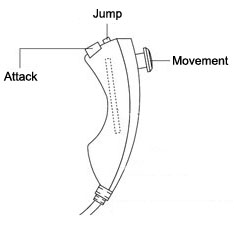
\includegraphics[scale=0.6]{Figures/nunchuk}
  \caption{Button assignments}
  \label{fig:Nunchuk} 
\end{figure}
>>>>>>> origin/master

We assigned the thumbstick to move horizontally and duck. The two buttons at the top are used to jump
and attack. These buttons assignments was the combination that felt most comfortable.

\section{Graphics}
Gameduino...

\subsection{Assets}
Assets...

\subsection{Sound} %Cebrail/Jonathan

We implemented sound effects on essential events. We Agreed that it was what the game needed to give a better feel.\\
We decided that the sounds we wanted was from the hero, and when he interacts with something. We added a sounds for jumping, attacking, when exiting a map and when collecting a coin.\\
To include bacground music we would have needed about 2kb more space in the flash memory since it takes alot of code to make this work. A solution would have been to use a shorter music file in the GD2 file and looping it, but we agreed that it would be annoying and steered clear of it.

